\subsection{Image Analysis}
	Image analysis is the use of various techniques such as pattern recognition, geometry calculations, and signal processing to extract information from digital images for later use. Image processing however is the application of various processes on an image to change or improve the way it looks. The processing stage normally comes before the analysis stage in an effort to simplify the analysis processes and improve their success.
	\subsubsection{Usages}
	Image processing and analysis has been applied to multiple areas with its value and effectiveness rapidly improving alongside camera technology and computing power. These applications include recognising faces in social media uploads \citep{zuckerberg2011tagging} to the utilisation of satellite imagery to tracking the changing shape of coastlines \citep{costalimagery}.
	\paragraph{Medical}
	Arguably one of the most important uses of image analysis, advances in medical imaging have reduced costs in healthcare, diagnosis time, recovery time, and improved the ability to localise and personalise treatments \citep{esfmedical}. Major uses of image analysis in medical applications are the use of Magnetic Resonance Imaging (MRI) and Computerised Topography Scanning (CT Scan) to create detailed images of the human body and identify illness before some symptoms arise.
	\begin{figure}[h!]
		\centering
		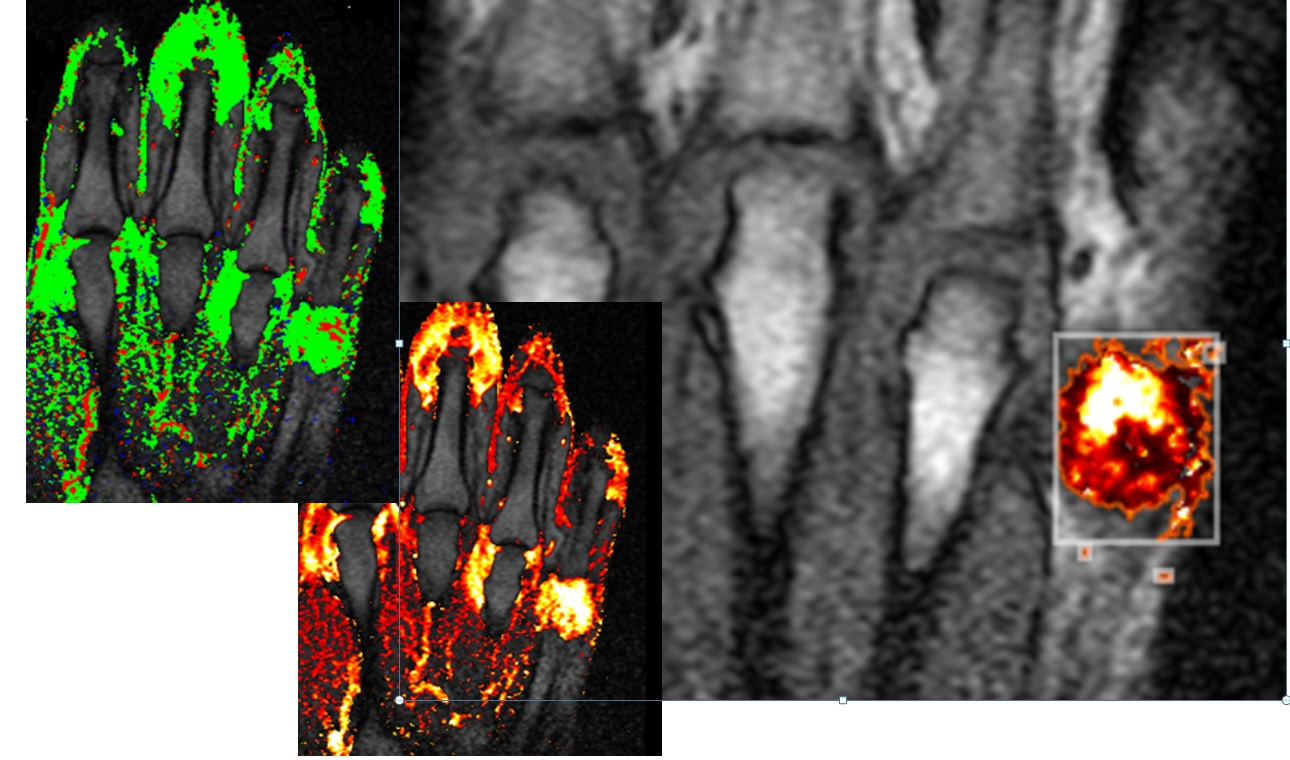
\includegraphics[width=10cm]{../images/mri.jpg}
		\caption{Identification of arthritis in an MRI scan \citep{mriimage}}			
		\label{fig:mri}
	\end{figure}
	\paragraph{Transport}
	Image analysis has been included in the consumer automotive market on various models since 2004 when Honda introduced an thermographic night vision camera with pedestrian detection on the Legend  \citep{hondanightvision}. Since this initial introduction many vehicle manufacturers have included image analysis and recognition features as options such as speed limit sign recognition, lane departure warning systems, and automatic braking systems based on hazard recognition.
	\paragraph{Engineering}
	\paragraph{Space}